\section{Modellering}
\subsection{Modell 1}
I den første modellen demonstererr vi dempingen som de forskjellig frekvenskomponentene i et signal opplever når det sendes gjennom et medium. Dette gjøres ved å sende et signal med flere frekvenskomponenter gjennom en dempende funksjon, og deretter analysere hvordan de forskjellige komponentene blir påvirket.
Vi tar utgangspunkt i en firkantpuls med periode $T$:
\[
    V_{inn}(t) = \begin{cases}
        5, & -\frac{T}{2} \leq t < 0 \\
        0, & 0 \leq t < \frac{T}{2} \\
    \end{cases}, \quad hvor \quad T = 100ns,\qquad duty\ cycle = 50\%
\]
Vi bestemmer først Fourier-rekken til firkantpulsen for å finne frekvenskomponentene:
\[
    V_{inn}(t) = \sum_{n=1,3,5,...}^{\infty} c_n e^{j n \omega_0 t}, \quad hvor \quad \omega_0 = \frac{2\pi}{T}
\]
Merk at siden vi vet at duty cycle er 50\%, vil bare oddetalls harmoniske være tilstede i Fourier-rekken.
Koefisientene $c_n$ kan beregnes som:
\[
    c_n = \frac{1}{T} \int_{-T/2}^{T/2} V(t) e^{-j n \omega_0 t} dt = \frac{5}{T} \int_{-T/2}^{0} e^{-j n \omega_0 t} dt = \frac{5}{j n \pi} (1 - (-1)^n)
\]
Vi for dermed at:
\[
    V_{inn}(t) = \sum_{n=1,3,5,...}^{\infty} \frac{10}{j n \pi} e^{j n \omega_0 t}
\]
For å modellere dempingen i mediet, antar vi en en tilnærment lik realistiske verider for R, G, L og C:
\begin{figure}[h]
    \centering
    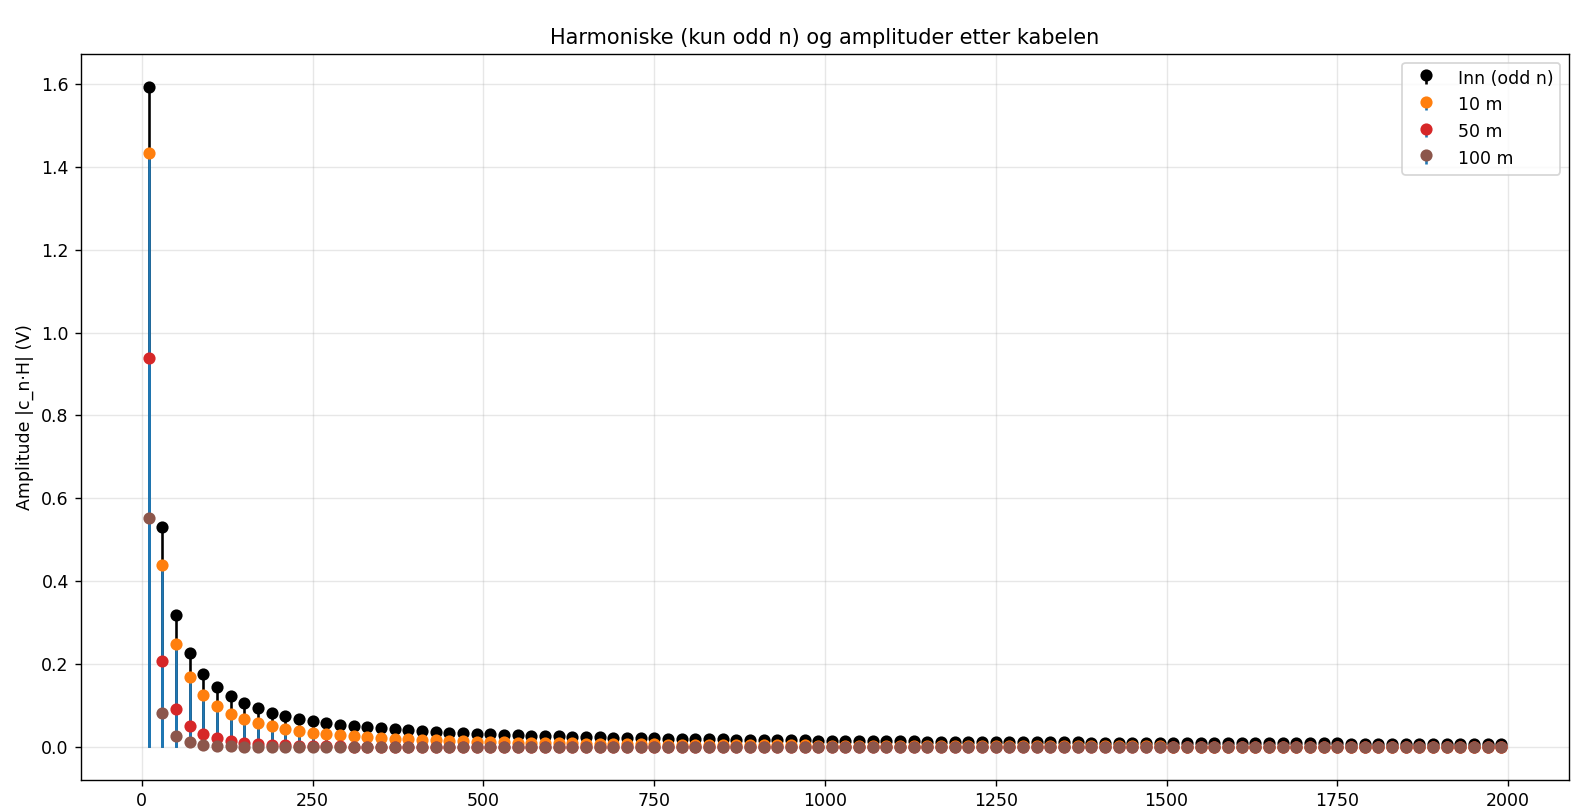
\includegraphics[width=1\textwidth]{Media/modellering1.png}
    \caption{Modell 1}
    \label{fig:modell1}
\end{figure}
